\documentclass[a4paper, 12pt]{article}

%%% Работа с русским языком
\usepackage{cmap}					% поиск в PDF
\usepackage{mathtext} 				% русские буквы в формулах
\usepackage[T2A]{fontenc}			% кодировка
\usepackage[utf8]{inputenc}			% кодировка исходного текста
\usepackage[russian]{babel}	% локализация и переносы

%%% Дополнительная работа с математикой
\usepackage{amsmath,amsfonts,amssymb,amsthm,mathtools} % AMS
\usepackage{icomma} % "Умная" запятая: $0,2$ --- число, $0, 2$ --- перечисление

%% Номера формул
%\mathtoolsset{showonlyrefs=true} % Показывать номера только у тех формул, на которые есть \eqref{} в тексте.

%% Шрифты
\usepackage{euscript}	 % Шрифт Евклид
\usepackage{mathrsfs} % Красивый матшрифт

%% Поля
\usepackage[left=2cm,right=2cm,top=2cm,bottom=2cm,bindingoffset=0cm]{geometry}

%% Русские списки
\usepackage{enumitem}
\makeatletter
\AddEnumerateCounter{\asbuk}{\russian@alph}{щ}
\makeatother

%%% Работа с картинками
\usepackage{graphicx}  % Для вставки рисунков
\graphicspath{{images/}{images2/}}  % папки с картинками
\setlength\fboxsep{3pt} % Отступ рамки \fbox{} от рисунка
\setlength\fboxrule{1pt} % Толщина линий рамки \fbox{}
\usepackage{wrapfig} % Обтекание рисунков и таблиц текстом

%%% Работа с таблицами
\usepackage{array,tabularx,tabulary,booktabs} % Дополнительная работа с таблицами
\usepackage{longtable}  % Длинные таблицы
\usepackage{multirow} % Слияние строк в таблице

%% Красная строка
\setlength{\parindent}{2em}

%% Интервалы
\linespread{1}
\usepackage{multirow}

%% TikZ
\usepackage{tikz}
\usetikzlibrary{graphs,graphs.standard}

%% Верхний колонтитул
\usepackage{fancyhdr}
\pagestyle{fancy}

%% Перенос знаков в формулах (по Львовскому)
\newcommand*{\hm}[1]{#1\nobreak\discretionary{}
	{\hbox{$\mathsurround=0pt #1$}}{}}

%% Мои дополнения
\usepackage{float} %Добавляет возможность работы с командой [H] которая улучшает расположение на странице
\usepackage{gensymb} %Красивые градусы
\usepackage{graphicx}               % Импорт изображений
\usepackage{caption} % Пакет для подписей к рисункам, в частности, для работы caption*


\begin{document}

\newcommand{\HRule}{\rule{\linewidth}{0.7mm}} % Defines a new command for the horizontal lines, change thickness here
	
	\begin{center}
		\large\textbf{Московский Физико-Технический Институт}\\
		\large\textbf{(государственный университет)}
	
		\vfill
		
		\Large Лабораторная работа по курсу общей физики № 3.2.8\\[0.5cm] % Minor heading such as course title
		
		%----------------------------------------------------------------------------------------
		%	TITLE SECTION
		%----------------------------------------------------------------------------------------
		
		\HRule
		\\[0.4cm]
		{ \huge \bfseries Релаксационные колебания}
		\\[0.4cm] % Title of your document
		\HRule
		\\[0.5cm]
		
		\ \\
	\textbf{\large Автор:} \\	
	\large Баранников Андрей Б01-001\\
		\vfill
		\hspace*{-0.8 cm}
\includegraphics[width=100 pt]{frkt_logo}\\
		\large Долгопрудный, 2021
	\end{center}

\newpage
\setcounter{page}{2}
\fancyfoot[c]{\thepage}
\fancyhead[L] {Работа 3.2.8}
\fancyhead[R]{}

\textbf{Цель работы:} определить характеристики шарообразных неодимовых магнитов и, используя законы взаимодействия магнитных моментов с полем, измерить горизонтальную и вертикальную составляющие индукции магнитного поля Земли и магнитное наклонение.

\textbf{В работе используются:} 12 одинаковых неодимовых магнитных шариков, тонкая нить для изготовления крутильного маятника, медная проволока диаметром (0,5 – 0,6) мм, электронные весы, секундомер, измеритель магнитной индукции АТЕ-8702, штангенциркуль, брусок из немагнитного материала (25$\times$30$\times$60 мм$^3$), деревянная линейка, штатив из немагнитного материала; дополнительные неодимовые магнитные шарики ($\thicksim$ 20 шт.) и неодимовые магниты в форме параллелепипедов (2 шт.), набор гирь и разновесов.

\section*{Экспериментальная установка}

\textbf{Измерение горизонтальной составляющей индукции магнитного поля Земли}


\begin{figure}[h!]
	\centering
	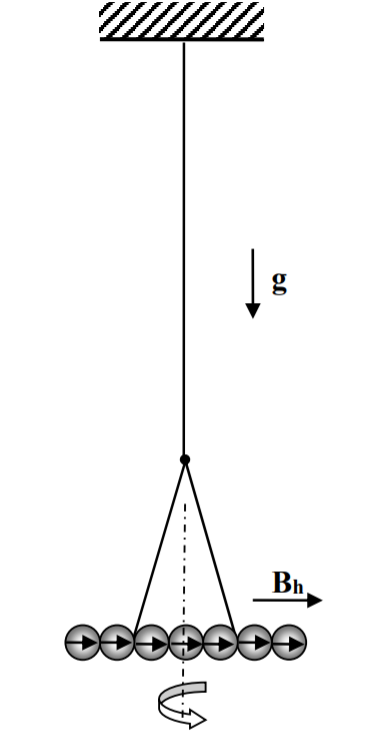
\includegraphics[scale=0.7]{image_1}
\end{figure}

Магнитное поле Земли в настоящей работе определяется по периоду крутильных колебаний магнитной стрелки вокруг вертикальной оси.

Магнитная стрелка» образована из сцепленных друг с другом противоположными полюсами шариков и с помощью $\Lambda$-образного подвеса подвешена в горизонтальном положении. Под действием вращательного момента магнитный момент «стрелки» выстроится вдоль горизонтальной составляющей магнитного поля Земли в направлении Юг → Север.

Период колебаний маятника оказывается пропорциональным числу шаров $n$, составляющих «стрелку»:

\begin{equation*}
	T(n) = n \cdot \pi\sqrt{\frac{md^2}{3P_mB_h}}.
\end{equation*}
\vspace{20mm}

\textbf{Измерение вертикальной составляющей индукции магнитного поля Земли.}

\begin{figure}[h!]
	\centering
	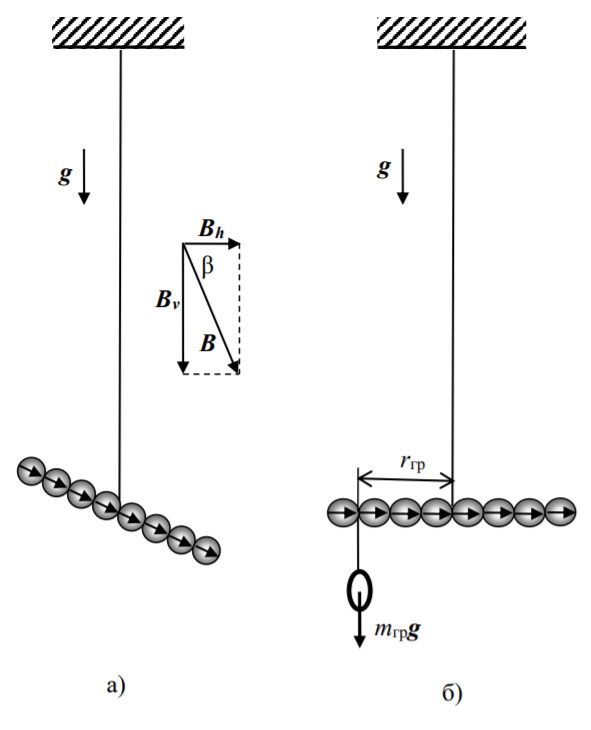
\includegraphics[scale=0.7]{image_2}
\end{figure}

Для измерения вертикальной составляющей вектора индукции поля Земли используется та же установка, что и для измерения горизонтальной составляющей с тем лишь отличием, что магнитная «стрелка» подвешивается на нити без $\Lambda$-образного подвеса. В этом случае магнитная «стрелка», составленная из чётного числа шариков и подвешенная на тонкой нити за середину, расположится не горизонтально, а под некоторым, отличным от нуля, углом к горизонту.

С помощью небольшого дополнительного грузика «стрелку» можно «выровнять», расположив её горизонтально: в этом случае момент силы тяжести груза относительно точки подвеса будет равен моменту сил, действующих на «стрелку» со стороны магнитного поля Земли.
\vspace{15mm}

Выпишем все необходимые формулы.

Сила взаимодействия двух небольших постоянных магнитов, направленных вдоль прямой, соединяющей их:

\begin{equation*}
	F = -6\frac{P_m^2}{r^4}
\end{equation*}

индукция магнитного поля $\overrightarrow{B_p}$ на полюсах однородно намагниченного шара связана с величиной намагниченности $\overrightarrow{p}_m$ и остаточной магнитной индукцией $\overrightarrow{B_r}$ формулой:

\begin{equation*}
	\overrightarrow{B_p} = (8\pi /3)\overrightarrow{p_m} = \frac{2}{3}\overrightarrow{B_r}.
\end{equation*}


В магнитном поле с индукцией $\overrightarrow{B}$ на точечный магнитный диполь $\overrightarrow{P_m}$ действует механический момент сил:

\begin{equation*}
	\overrightarrow{M} = \overrightarrow{P_m} \times \overrightarrow{B}
\end{equation*}

Период колебаний крутильного маятника в зависимости от количества шаров:

\begin{equation*}
	T(n) = n \cdot \pi\sqrt{\frac{md^2}{3P_mB_h}}
\end{equation*}

Момент силы тяжести, уравновешивающего груза в зависимости от количества шаров:

\begin{equation*}
	M(n) = n \cdot P_mB_{\nu}
\end{equation*}

\section*{{Ход работы}}
\subsection*{Задание № 1. Метод А.}
\begin{enumerate}
\item Взвесим шарики и измерим диаметр. В результате $m = 0,876 \ г; \ d = 6 \ мм$ \\
\item Выясним, на каком максимальном расстоянии шарики удерживают друг друга в поле тяжести Земли. $r_{max} = 17 \ мм$\\
\item Рассчитаем величину магнитного момента магнитика $P_m$:\\
\[
F = \frac{6P_m^2}{r_{max}^4} = mg \quad \Rightarrow \quad \boxed{P_m = r_{max}^2 \sqrt{\frac{mg}{6}} = (1,7 \ см)^2 \sqrt{\frac{0,876 \ г \cdot 980 \ см/с^2}{6}} = 34,57 \ эрг/Гс }
\]
\item Рассчитаем величину намагниченности материала шариков:
\[
\boxed{p_m = P_m/V = \frac{34,57 \ эрг/Гс }{\frac{4}{3} \pi \cdot 0,3^3\ cм^3} \approx 305 \ Гс}
\]

\item Рассчитаем величину $B_p$ магнитного поля на полюсах шарика и сравним расчётное значение с измеренным: \\
\[
\boxed{B_p = \frac{2P_m}{R^3} = \frac{2 \cdot 34,57 \ эрг/Гс }{0,3^3 \ см^3} \approx 2,56 \ кГс}
\]
Значение, измеренное с помощью магнетометра ATE-8702: \\
\[
\boxed{B_p = 194 \ мТ = 1,94 \ кГс}
\]
\item Рассчитаю величину остаточной магнитной индукции: \\
\[
\boxed{B_r = 4\pi p_m = 4\pi \cdot 305 \ Гс \approx 3,8 \ кГс}
\]


\subsection*{Задание № 1. Метод B.}
\item  Минимальный вес $F$ системы с цепочки с гирей, при котором она отрывается от верхнего шарика: \\
\[
F = 3,136 \ Н \quad \Rightarrow \quad
F_0 = \frac{F}{1,08} \approx 2,9 \ H
\]
\item 
\[
F_0 = \frac{6 P_m^2}{d^4} \quad \Rightarrow \quad \boxed{P_m = \sqrt{\frac{F_0 \cdot d^4}{6}} = \sqrt{\frac{2,9 \cdot 10^5 \ дин \cdot 0,6^4 \ см^4 }{6}} \approx 80 \ эрг/Гс}
\]
\item Рассчитаю величину поля на полюсах: \\
\[
\boxed{B_p = \frac{2P_m}{R^3} = \frac{2 \cdot 80 \ эрг/Гс }{0,3^3 \ см^3} \approx 5,93 \ кГс}
\]
\item По результатам вычисления магнитных моментов \textbf{точнее всего оказался  \\ Метод А.}

\subsection*{Задание № 2}
\item Оценим влияние упругости нити на период колебаний, для этого свернём стрелку в кольцо и возбудим крутильные колебания. В таком случае период колебаний будет $T =  136,4 \ c \ $ Очевидно,  упругостью можно пренебречь.
\item Измерим зависимость $T(n)$

\begin{table}[!h]
	\centering
	\begin{tabular}{|c|c|c|c|c|c|c|}
		\hline
		n    & 3    & 5    & 7    & 9    & 11   & 12   \\ \hline
		T, c & 0,92 & 1,51 & 2,18 & 2,80 & 3,35 & 3,76 \\ \hline
	\end{tabular}
	\caption{Зависимость периода колебаний T от количества магнитных шариков n}
	\label{tab:table_1}
\end{table}

\item Построю график $T(n)$:
\begin{figure}[h!]
	\centering
	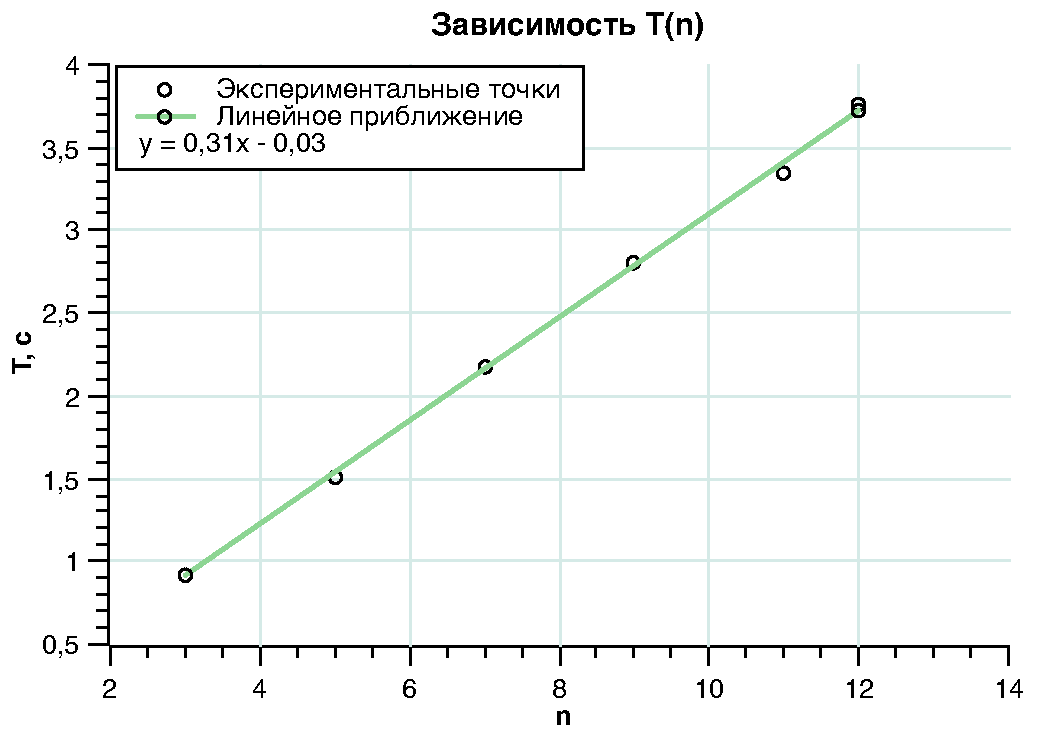
\includegraphics[scale=0.5]{plot_1}
	\caption{График экспериментальной зависимости T(n)}
	\label{fig:plot_1}
\end{figure}


\item Аппроксимирую  экспериментлаьную зависимость T(n): \\
Получилась прямая T = 0,31n, соответсвенно, коэффициент наклона k = 0,31 \\
\item Рассчитаем величину горизонтальной составляющей магнитного поля Земли: \\
\[
B_h = \pi^2 m d^2 / 3 k^2 P_m = \frac{\pi^2 \cdot 0,876 \ г \cdot 0,36 \ см^2}{3 \cdot  0,0961 \cdot  34,57 \ эрг/с} =  0,3 \ Гс
\]

\section*{Задание № 3}
\item Уравновесим магнитные стрелки при разном значении количества шариков n. Результаты сведём в таблицу: \\

\begin{table}[!h]
	\centering
	\begin{tabular}{|c|c|c|c|}
		\hline
		n  & l & m, г  & M, дин/см \\ \hline
		4  & 1 & 0,182 & 107,0     \\ \hline
		6  & 2 & 0,202 & 237,6     \\ \hline
		8  & 2 & 0,250 & 294,0     \\ \hline
		10 & 3 & 0,195 & 344,0     \\ \hline
		12 & 3 & 0,225 & 396,9     \\ \hline
	\end{tabular}
	\caption{Зависимость механического момента M от количества магнитных шариков n}
	\label{tab:table_2}
\end{table}

\item Построю график M = M(n):\\

\begin{figure}[h!]
	\centering
	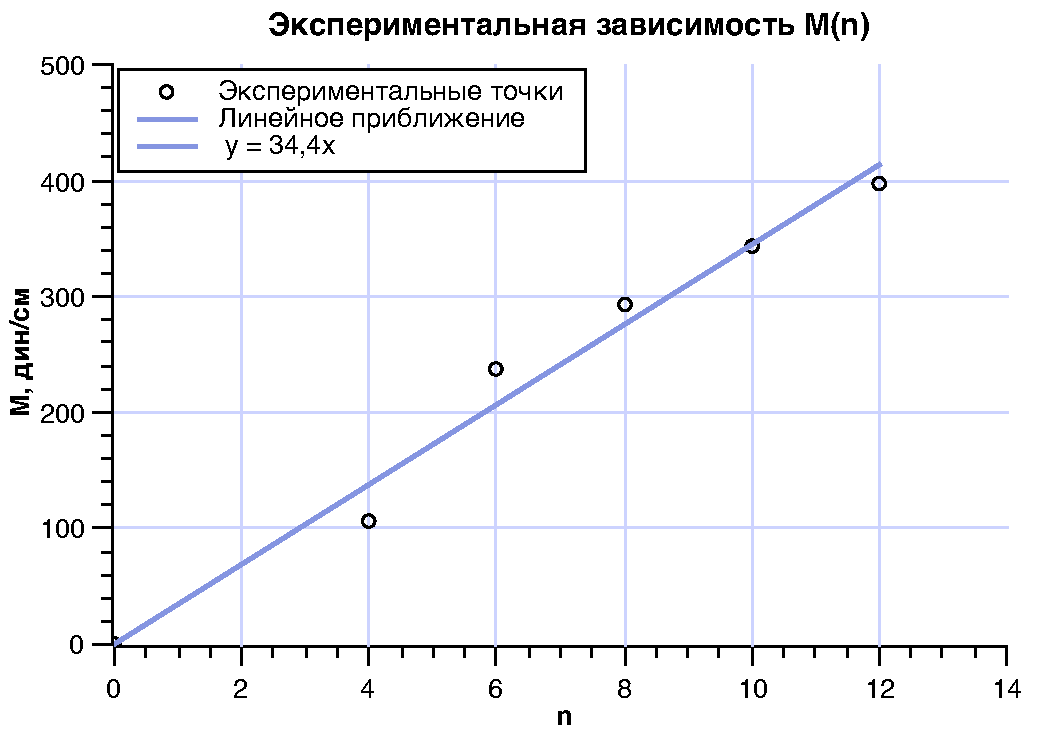
\includegraphics[width= 0.8\textwidth]{plot_2}
	\caption{График экспериментальной зависимости M(n)}
	\label{fig:plot_2}
\end{figure}

\item При аппроксимации экспериментальной зависимсости M(n) прямой линией \\ получается:\\
M = 34,4x, соответсвенно, коэффициент наклона $A = 34,4 \ дин \cdot см$  \\
\item Рассчитаю величину $B_{\nu}$: \\
\[
B_{\nu} = \frac{A}{P_m} \approx 0,78 \ Гс
\]
\item Итоговая индукция магнитного поля Земли $\boxed{B = \sqrt{B_{\nu}^2 + B_h^2} = 0,83 \ Гс}$ \\
Магнитное отклонение $\boxed{\beta = \arctg \frac{B_{\nu}}{B_h} = 68^{\circ}}$ \\
Магнитное поле на широте Долгопрудного по таблице: $\boxed{B_{табл} = 50 \ Гс}$

\end{enumerate}

\end{document}